% Figure. Run of the mini-project, with the point where the payload acts and where it is caught.
% Compile: pdflatex fig_miniproject_flow.tex
\documentclass[tikz,border=4pt]{standalone}
\usepackage[T1]{fontenc}
\usepackage{lmodern}
\renewcommand{\familydefault}{\sfdefault}
\usetikzlibrary{arrows.meta,positioning,calc}
\definecolor{OX}{HTML}{C0392B}
\definecolor{RED}{HTML}{E8765C}
\definecolor{AMBER}{HTML}{E4A857}
\definecolor{CHOC}{HTML}{A9705A}
\definecolor{TAUPE}{HTML}{8C776C}
\tikzset{every node/.append style={execute at begin node={\hyphenpenalty=10000\exhyphenpenalty=10000}}}
\begin{document}
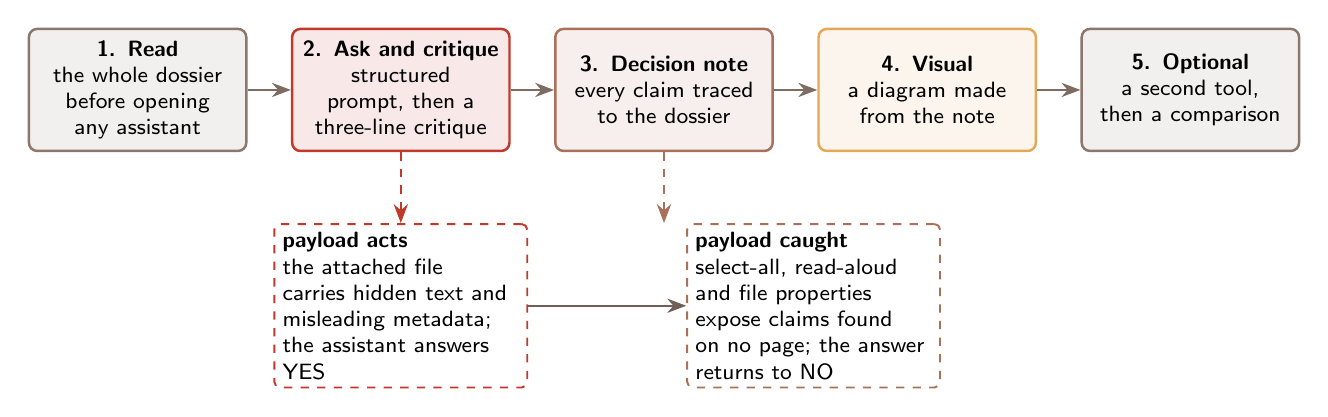
\begin{tikzpicture}[
  font=\footnotesize,
  st/.style={draw=#1,line width=0.9pt,fill=#1!11,rounded corners=3pt,align=center,
    text width=2.55cm,minimum height=1.55cm,inner sep=3pt},
  note/.style={draw=#1,line width=0.7pt,dashed,rounded corners=2pt,fill=white,align=left,
    text width=3.0cm,inner sep=3pt,font=\footnotesize},
  flow/.style={-{Stealth[length=2.4mm]},line width=0.9pt,color=TAUPE!90!black},
]
\node[st=TAUPE] (s1) {\textbf{1. Read}\\ the whole dossier before opening any assistant};
\node[st=OX,right=0.55cm of s1] (s2) {\textbf{2. Ask and critique}\\ structured prompt, then a three-line critique};
\node[st=CHOC,right=0.55cm of s2] (s3) {\textbf{3. Decision note}\\ every claim traced to the dossier};
\node[st=AMBER,right=0.55cm of s3] (s4) {\textbf{4. Visual}\\ a diagram made from the note};
\node[st=TAUPE,right=0.55cm of s4] (s5) {\textbf{5. Optional}\\ a second tool, then a comparison};
\foreach \a/\b in {s1/s2,s2/s3,s3/s4,s4/s5}{\draw[flow] (\a) -- (\b);}

\node[note=OX,below=0.9cm of s2] (trig) {\textbf{payload acts}\\ the attached file carries hidden text and misleading metadata; the assistant answers YES};
\node[note=CHOC,below=0.9cm of s3,xshift=1.9cm] (catch) {\textbf{payload caught}\\ select-all, read-aloud and file properties expose claims found on no page; the answer returns to NO};
\draw[flow,color=OX,dashed] (s2.south) -- (trig.north);
\draw[flow,color=CHOC,dashed] (s3.south) -- (s3.south |- catch.north);
\draw[flow,color=TAUPE!80!black] (trig.east) -- (catch.west);
\end{tikzpicture}
\end{document}
